% -----------------------------------------------------------------------------
% File: main.tex
% Description: Main entry point for the modular final LaTeX report.
% -----------------------------------------------------------------------------

\documentclass[12pt]{article}

% --- Custom Style & Settings ---
% -----------------------------------------------------------------------------
% File: settings/packages.tex
% Description: Centralized package imports for the report.
% -----------------------------------------------------------------------------

% --- Mathematics ---
\usepackage{amsmath}
\usepackage{amssymb}
\usepackage{amsfonts}
\usepackage{mathtools}

% --- Layout & Geometry ---
\usepackage{geometry}
\geometry{
    a4paper,
    top=2.0cm,
    bottom=2.0cm,
    left=1.6cm,
    right=1.6cm,
    columnsep=0.6cm
}

% --- Fonts & Typography ---
\usepackage[utf8]{inputenc}
\usepackage[T1]{fontenc}
\usepackage{microtype}
\usepackage{newtxtext,newtxmath} % Standard Times Roman font for papers

% --- Figures & Tables ---
\usepackage{graphicx}
\usepackage{booktabs}
\usepackage{colortbl}
\usepackage{caption}
\usepackage{subcaption}
\usepackage{float}
\usepackage{multirow}

% --- TikZ & Visualization ---
\usepackage{tikz}
\usetikzlibrary{shapes, shapes.geometric, arrows, positioning, fit, calc, shadows}
\usepackage{pgfplots}
\pgfplotsset{compat=1.18}

% --- Code Highlighting ---
\usepackage{listings}
\usepackage{xcolor}

% --- Hyperlinks & Referencing ---
\usepackage{hyperref}
\hypersetup{
    colorlinks=true,
    linkcolor=techBlue,
    citecolor=codeGreen,
    urlcolor=techBlue
}

% --- Bibliography ---
\usepackage[style=ieee, backend=biber]{biblatex}
\addbibresource{bib/references.bib}

\usepackage{settings/styles}
% -----------------------------------------------------------------------------
% File: settings/commands.tex
% Description: Custom colors, operators, and formatting helpers.
% -----------------------------------------------------------------------------

% --- Color System ---
\definecolor{techBlue}{RGB}{10, 80, 160}
\definecolor{darkBlue}{RGB}{5, 40, 90}
\definecolor{alertRed}{RGB}{190, 30, 30}
\definecolor{codeGreen}{RGB}{0, 130, 60}
\definecolor{lightGray}{RGB}{245, 245, 245}
\definecolor{borderGray}{RGB}{210, 210, 210}

% --- Text Decorators ---
\newcommand{\highlight}[1]{\textbf{\textcolor{techBlue}{#1}}}
\newcommand{\keyterm}[1]{\textbf{\textcolor{darkBlue}{#1}}}
\newcommand{\todo}[1]{\textcolor{alertRed}{\textbf{[TODO: #1]}}}

% --- Code Block Styles ---
\lstset{
    backgroundcolor=\color{lightGray},
    basicstyle=\ttfamily\scriptsize,
    breaklines=true,
    frame=single,
    rulecolor=\color{borderGray},
    numbers=left,
    numberstyle=\tiny\color{gray},
    keywordstyle=\color{techBlue}\bfseries,
    commentstyle=\color{codeGreen}\itshape,
    stringstyle=\color{alertRed},
    showstringspaces=false,
    captionpos=b
}

% --- Custom Macros ---
\newcommand{\paperCard}[3]{
    \noindent\colorbox{lightGray}{
        \parbox{\linewidth}{
            \vspace{0.2em}
            \small\highlight{#1} \\
            \scriptsize \textit{#2} \hfill \textbf{#3}
            \vspace{0.2em}
        }
    }
    \vspace{0.8em}
}

\newcommand{\resultBox}[2]{
    \noindent\colorbox{lightGray}{
        \parbox{\linewidth}{
            \centering
            \vspace{0.3em}
            \scriptsize #1 \\
            \large\textbf{#2}
            \vspace{0.3em}
        }
    }
}


% --- Graphics Paths ---
\graphicspath{ {./images/} {./figures/} }

% --- Title Block Metadata ---
\title{
    \large\textbf{Introduction to Data Science: Final Project Report} \\
    \vspace{0.4em}
    \LARGE\highlight{Critical Analysis of Advanced Deep Learning in Medical Imaging \& Automated Software Engineering}
}

\author{
    \normalsize
    \begin{tabular}{c c}
        \textbf{Hoang Khang Nguyen} & \textbf{Duy Thanh Nguyen} \\
        \scriptsize Student ID: 25C01035 & \scriptsize Student ID: 25C01047 \\
        \scriptsize Email: \href{mailto:25C01035@student.hcmus.edu.vn}{\texttt{25C01035@student.hcmus.edu.vn}} & \scriptsize Email: \href{mailto:25C01047@student.hcmus.edu.vn}{\texttt{25C01047@student.hcmus.edu.vn}} \\
        & \\
        \textbf{Nguyen Nang Khanh Vu} & \textbf{Nguyen Huu Hung Mai} \\
        \scriptsize Student ID: 25C01036 & \scriptsize Student ID: 25C01032 \\
        \scriptsize Email: \href{mailto:25C01036@student.hcmus.edu.vn}{\texttt{25C01036@student.hcmus.edu.vn}} & \scriptsize Email: \href{mailto:25C01032@student.hcmus.edu.vn}{\texttt{25C01032@student.hcmus.edu.vn}}
    \end{tabular}
    \\[1.5em]
    \small Master of Data Science \\
    \small\textbf{University of Science, VNU-HCM}
}

\date{\small\today}

\begin{document}

% Compile Title
\maketitle

% Abstract (Single-column layout using strip if needed, or simply standard abstract in twocolumn)
\begin{abstract}
This report presents a comprehensive analysis and synthesis of three state-of-the-art research papers presented at the International Conference on Computational Collective Intelligence (ICCCI 2025). The selected papers address key challenges at the intersection of artificial intelligence, clinical diagnostics, and automated software engineering: (1) leukemia blast cell detection using YOLOv11 with the GCLI attention module, achieving 25.1\% mAP50-95 with 11\% parameter reduction; (2) Alzheimer's disease diagnosis using VGG16 with dual-model disjunction fusion, reaching 89.87\% accuracy and 87.50\% sensitivity; and (3) LLM-based code quality review, where Claude 3.5 Sonnet aligns with human expert consensus in 9 out of 12 metrics. For each paper, we present the research background, proposed methodology, dataset description, experimental results with detailed analysis, and key contributions. We conclude with cross-domain observations on data integrity, sensitivity--precision trade-offs, and the effectiveness of lightweight domain-specific approaches versus heavyweight general-purpose methods.
\end{abstract}

\vspace{1em}

% --- Section 1: Introduction ---
% -----------------------------------------------------------------------------
% File: sections/01_introduction.tex
% Description: Section 1 - General Introduction
% -----------------------------------------------------------------------------

\section{General Introduction}
\label{sec:intro}

\subsection{Context and Research Motivation}

The rapid convergence of deep learning architectures and large language models (LLMs) has catalyzed a paradigm shift across diverse industrial and scientific domains. Among these, two fields stand out for their critical importance, high standards of accuracy, and unique engineering challenges: \highlight{Computer-Aided Diagnosis (CAD)} in medical imaging and \highlight{Automated Software Engineering (ASE)} in software development.

In medical imaging, particularly in hematological oncology and neurodegenerative disease screening, deep learning has transitioned from an experimental tool to a clinical necessity. The diagnosis of diseases like leukemia and Alzheimer's relies heavily on high-precision analysis of visual data, such as peripheral blood smear images and magnetic resonance imaging (MRI) scans. However, manual examination of these materials is notoriously time-consuming, prone to subjective variance, and constrained by a global shortage of clinical specialists. The main challenges here are visual: distinguishing subtle cellular morphology aberrations and detecting localized structural brain tissue shrinkage (atrophy) from high-dimensional scans.

Concurrently, automated software engineering has entered a new era driven by generative artificial intelligence. Code review, which has historically been a human-centric bottleneck in the software development lifecycle (SDLC), is being automated using LLMs as code review agents. This paradigm promises to dramatically reduce developer overhead, accelerate time-to-market, and enforce consistent code quality standards. Nevertheless, deploying LLM agents in production software environments introduces critical questions regarding scoring consistency, domain alignment, data privacy, and the trade-off between API costs and actual quality improvements.

\subsection{Report Objectives}

This report presents a comprehensive analysis and synthesis of three state-of-the-art research papers presented at the International Conference on Computational Collective Intelligence (ICCCI 2025), addressing the above challenges:
\begin{enumerate}
    \item \highlight{Leukemia Detection Based on YOLOv11 with Global and Local Contexts Interaction} \cite{leukemia_gcli_2025}: proposes integrating a lightweight attention module (GCLI) into the YOLOv11 architecture to improve blast cell detection in peripheral blood smear images.
    \item \highlight{The New Method for Detection of Alzheimer's Disease} \cite{alzheimer_vgg_2025}: explores subject-level MRI classification using progressive transfer learning with VGG16 and a dual-model disjunction fusion strategy.
    \item \highlight{LLMs as Code Review Agents: A Rapid Review and Experimental Evaluation with Human Expert Judges} \cite{llm_review_2025}: conducts a comparative analysis evaluating LLM-generated code quality scores against senior developer consensus across 12 quality metrics.
\end{enumerate}

For each paper, we present the research background, the proposed methodology, the experimental setup and dataset, and a detailed analysis of the results. We conclude each section with remarks on the paper's contributions and limitations.


% --- Section 2: Leukemia Detection ---
% -----------------------------------------------------------------------------
% File: sections/02_leukemia_detection.tex
% Description: Section 2 - Leukemia Detection Based on YOLOv11 with GCLI
% -----------------------------------------------------------------------------

\section{Paper 1: Leukemia Detection Based on YOLOv11 with GCLI}
\label{sec:leukemia}

\paperCard{Leukemia Detection Based on YOLOv11 with Global and Local Contexts Interaction}{Minh Tai Pham Nguyen, Trong Nhan Le, Minh Khue Pham Tran}{ICCCI 2025, LNAI 16139, pp. 231--242}

\subsection{Background and Research Motivation}
Leukemia is a group of malignant cancers originating in the bone marrow, characterized by the uncontrolled proliferation of abnormal, immature white blood cells (blasts). According to global cancer statistics, leukemia accounts for approximately 2.5\% of all cancers worldwide and is classified into four main types: Acute Myeloid Leukemia (AML), Chronic Myeloid Leukemia (CML), Acute Lymphocytic Leukemia (ALL), and Chronic Lymphocytic Leukemia (CLL).

Early detection of leukemia plays a crucial role in the treatment process. However, this is an extremely challenging problem in deep learning-based medical imaging because malignant blast cells often share very similar morphology with healthy mature leukocytes (e.g., lymphocytes and monocytes) on peripheral blood smear images. This makes it difficult for conventional convolutional neural networks (CNNs) to distinguish between normal and abnormal cells without capturing both local features (e.g., chromatin texture, nucleus-to-cytoplasm ratio) and global features (e.g., cellular density, spatial distribution patterns).

Computer-Aided Diagnosis (CAD) systems leveraging deep learning have been proposed to assist medical professionals in preliminary screening, improving both the speed and accuracy of the diagnostic process.

\subsection{Paper Objectives}
The paper proposes integrating a \highlight{Global Context and Local Interaction (GCLI)} module into the YOLOv11 architecture to improve leukemia blast cell detection. The specific objectives include:
\begin{itemize}
    \item Replacing the C2PSA (Position-Sensitive Attention) block in the baseline YOLOv11 with the GCLI module.
    \item Leveraging the ability to capture long-range dependencies and global--local feature interaction to better distinguish abnormal cells.
    \item Reducing the parameter count and computational cost compared to the baseline model.
\end{itemize}

\subsection{Proposed Method}

\subsubsection{The GCLI Module (Global Context and Local Interaction)}
The GCLI module is built upon the Global Context (GC) block and enhanced with local interaction techniques to improve attention weight generation. The key improvements of GCLI over the traditional GC block are:
\begin{itemize}
    \item \textbf{Replacing 2D bottleneck convolutions with 1D convolutions} using large kernels, which avoids dimensionality reduction and preserves rich feature information.
    \item \textbf{Dual-branch global pooling:} simultaneously applying Global Average Pooling (GAP, for noise suppression) and Global Max Pooling (GMP, for extracting salient features), combining their outputs ($2 \times 1 \times C/2$) before feeding into Conv1D $7\times7$.
    \item \textbf{SiLU activation function:} inserted between two 1D convolutions to optimize attention weight computation in complex feature spaces.
    \item \textbf{Partial feature utilization:} using only half of the channels ($C/2$) for attention weight generation, minimizing weighted redundancies.
\end{itemize}

\subsubsection{Mathematical Formulation}
The GCLI module processes an input feature map $X \in \mathbb{R}^{W \times H \times C}$ through a multi-stage pipeline:
\begin{enumerate}
    \item \textbf{Split Strategy:} The input channels are divided into two equal parts:
    \begin{equation}
        X_1, X_2 = \text{Split}(X) \quad \text{where } X_1, X_2 \in \mathbb{R}^{W \times H \times \frac{C}{2}}
    \end{equation}
    $X_1$ acts as an identity (frozen) branch to maintain spatial features, while $X_2$ undergoes attention modulation.

    \item \textbf{Global Context Modeling:} Long-range spatial dependencies are extracted from $X_2$ using a query-like projection:
    \begin{align}
        A &= \text{Softmax}(\text{Conv2D}_{1\times1}(X_2)) \in \mathbb{R}^{W \times H \times 1} \\
        X_{global} &= X_2 \otimes A \in \mathbb{R}^{W \times H \times \frac{C}{2}}
    \end{align}
    where $\otimes$ denotes matrix multiplication mapping spatial dependencies.

    \item \textbf{Local Channel Interaction:} The module computes a global descriptor via dual pooling and models local context via sequential 1D Convolutions:
    \begin{equation}
        Y = \text{GAP}(X_{global}) + \text{GMP}(X_{global}) \in \mathbb{R}^{1 \times 1 \times \frac{C}{2}}
    \end{equation}
    \begin{equation}
        S = \sigma\left(\text{Conv1D}_{3}\left(\text{SiLU}\left(\text{Conv1D}_{7}(Y)\right)\right)\right) \in \mathbb{R}^{1 \times 1 \times \frac{C}{2}}
    \end{equation}
    where $\sigma$ is the sigmoid function. The kernel sizes ($7\times7$ and $3\times3$) capture local multi-scale relationships.

    \item \textbf{Feature Modulation \& Concatenation:} The final modulated output is:
    \begin{align}
        X'_2 &= X_2 \odot S \\
        X_{out} &= \text{Concat}(X_1, X'_2) \in \mathbb{R}^{W \times H \times C}
    \end{align}
    where $\odot$ represents channel-wise multiplication.
\end{enumerate}

\pgfdeclarelayer{background}
\pgfsetlayers{background,main}
\begin{figure}[h]
    \centering
    \resizebox{0.95\textwidth}{!}{%
    \begin{tikzpicture}[
        node distance=0.4cm and 0.8cm,
        font=\sffamily\footnotesize,
        tensor/.style={rectangle, draw=black, fill=white, thick, minimum height=0.6cm, minimum width=1.2cm, align=center, font=\scriptsize},
        op/.style={circle, draw=black, thick, fill=white, inner sep=1pt, minimum size=0.6cm},
        block/.style={rectangle, draw=black, thick, fill=gray!10, rounded corners=2pt, minimum height=0.8cm, minimum width=1.8cm, align=center},
        groupbox/.style={rectangle, draw=gray, dashed, inner sep=0.3cm, rounded corners=5pt},
        arrow/.style={->, >=stealth, thick, techBlue, rounded corners=3pt}
    ]
        \node[tensor, fill=green!10] (input) {Input\\$W \times H \times C$};
        \coordinate[right=0.8cm of input] (split);
        \node[tensor, above right=1.5cm and 1.0cm of split, fill=gray!10] (part1) {Part 1 (Identity)\\$C/2$};
        \node[block, right=0.5cm of split, fill=red!10, yshift=-0.5cm] (conv2d) {Conv2D\\$1\times1$};
        \node[block, right=0.5cm of conv2d, fill=red!10] (softmax) {Softmax};
        \node[op, below=0.4cm of softmax] (mul1) {$\times$};
        \draw[arrow] (split) -- ++(0.2, -0.5) |- (conv2d.west);
        \draw[arrow] (conv2d) -- (softmax);
        \draw[arrow] (softmax) -- (mul1);
        \draw[arrow] (split) -- ++(0.2, -0.5) |- (mul1.west);
        \node[tensor, right=0.8cm of mul1] (pools) {GAP + GMP\\(Dual Pool)};
        \node[block, right=0.5cm of pools, fill=yellow!15] (conv1d_7) {Conv1D\\$7\times7$};
        \node[block, right=0.3cm of conv1d_7, fill=yellow!15] (silu) {SiLU};
        \node[block, right=0.3cm of silu, fill=yellow!15] (conv1d_3) {Conv1D\\$3\times3$};
        \node[block, right=0.3cm of conv1d_3, fill=blue!10] (sigmoid) {$\sigma(\cdot)$};
        \draw[arrow] (mul1) -- (pools);
        \draw[arrow] (pools) -- (conv1d_7);
        \draw[arrow] (conv1d_7) -- (silu);
        \draw[arrow] (silu) -- (conv1d_3);
        \draw[arrow] (conv1d_3) -- (sigmoid);
        \node[op, right=0.5cm of sigmoid] (mul2) {$\times$};
        \node[tensor, right=0.5cm of mul2, fill=purple!10] (concat) {Concat};
        \node[tensor, right=0.5cm of concat] (output) {Output\\$W \times H \times C$};
        \draw[arrow] (split) -- ++(0.2, -0.5) -- ++(0, -2.2) -| (mul2.south);
        \draw[arrow] (sigmoid) -- (mul2);
        \draw[arrow] (part1.east) -| (concat.north);
        \draw[arrow] (mul2) -- (concat);
        \draw[arrow] (concat) -- (output);
        \draw[arrow] (input) -- (split);
        \draw[arrow] (split) |- (part1);
        \begin{pgfonlayer}{background}
            \node[groupbox, fit=(conv2d) (softmax) (mul1), fill=red!2, label={[red]north:\scriptsize Global Context Modeling}] {};
            \node[groupbox, fit=(pools) (conv1d_7) (sigmoid), fill=yellow!2, label={[orange]south:\scriptsize Local Interaction (No Dim Reduction)}] {};
        \end{pgfonlayer}
    \end{tikzpicture}%
    }
    \caption{Architecture of the GCLI module. Channel splitting isolates features to focus learning on relevant context, while 1D Convolutions prevent information loss from dimensionality reduction.}
    \label{fig:gcli_architecture}
\end{figure}

\subsubsection{YOLOv11 Architecture with GCLI Integration}
YOLOv11 is one of the latest models in the YOLO family, inheriting important innovations such as Cross Stage Partial (CSP), the C3K2 feature extraction block, and the C2PSA block for self-attention. In the proposed architecture, the C2PSA block (combining PSA + C2f) is replaced by the GCLI module at the end of the feature extraction phase (backbone). Features processed through GCLI learn attention weights and are then passed to the feature synthesis phase (neck) for combination with multi-scale features. The GCLI module is positioned immediately after the Spatial Pyramid Pooling -- Fast (SPPF) block, enabling attention-guided features to propagate through the multi-scale Neck structure.

\subsection{Experiments and Results}

\subsubsection{LeukemiaAttri Dataset}
The LeukemiaAttri dataset (Rehman et al., 2024) is used for model evaluation. It is one of the most comprehensive and complex datasets for the leukemia detection problem:
\begin{itemize}
    \item \textbf{Total images:} 2,369 peripheral blood smear images at 3 magnification levels: 10x, 40x, and 100x.
    \item \textbf{Number of classes:} 14 leukemia classification categories, many of which share very similar visual characteristics.
    \item \textbf{Data split:} 1,677 training images and 692 test images (validation set is sampled from the training set).
    \item \textbf{Experimental setup:} 100x magnification images with top-down camera angle (angle 2).
\end{itemize}

\subsubsection{Experimental Results}
Table~\ref{tab:leukemia_results} presents the comparative performance of YOLOv11s models integrated with various attention modules on the LeukemiaAttri test set. Evaluation metrics include Sensitivity (recall), mAP50, mAP50-95, parameter count (Params), and GFLOPS.

\begin{table}[h]
    \centering
    \caption{Performance results of object detectors on the LeukemiaAttri test set.}
    \label{tab:leukemia_results}
    \resizebox{\linewidth}{!}{%
    \begin{tabular}{lccccc}
        \toprule
        \textbf{Model} & \textbf{Sens.} & \textbf{mAP50} & \textbf{mAP50-95} & \textbf{Params} & \textbf{GFLOPs} \\
        \midrule
        YOLOv11s & 48.9 & 38.8 & 22.6 & 9.41M & 21.3 \\
        YOLOv11s + ECA & 50.6 & 41.3 & 24.3 & 8.43M & 20.5 \\
        YOLOv11s + SE & 53.4 & \textbf{41.7} & 24.3 & 8.43M & 20.5 \\
        YOLOv11s + CBAM & \textbf{55.4} & 40.6 & 23.7 & 8.46M & 20.6 \\
        YOLOv11s + CA & 51.7 & 39.0 & 22.9 & 8.45M & 20.6 \\
        YOLOv11s + simAM & 51.5 & 40.2 & 23.4 & 8.43M & 20.5 \\
        YOLOv11s + GCB & 54.0 & 41.4 & 23.8 & 8.46M & 20.6 \\
        \rowcolor{techBlue!10}
        \textbf{YOLOv11s + GCLI} & 53.5 & 41.6 & \textbf{25.1} & \textbf{8.43M} & \textbf{20.5} \\
        \bottomrule
    \end{tabular}
    }
\end{table}

Detailed analysis of the results:
\begin{itemize}
    \item \textbf{Baseline YOLOv11s:} Achieves sensitivity of 48.9\%, mAP50 of 38.8\%, and mAP50-95 of 22.6\% with 9.41M parameters and 21.3 GFLOPS.
    \item \textbf{CBAM} achieves the highest sensitivity (55.4\%) thanks to its combination of channel and spatial attention, but mAP50-95 only reaches 23.7\%.
    \item \textbf{YOLOv11s + GCLI (proposed):} Achieves the highest mAP50-95 of \highlight{25.1\%}, surpassing all other attention modules in high-precision detection. Sensitivity reaches 53.5\% with only 8.43M parameters (a reduction of over 11\% compared to baseline) and 20.5 GFLOPS.
    \item \textbf{GCLI} maintains the same parameter count and FLOPS as ECA and simAM (the lightest in the group) while achieving the best overall detection accuracy.
\end{itemize}

\subsection{Conclusion and Contributions}
The paper proposes a YOLOv11 architecture integrating the GCLI module to replace the C2PSA block in the baseline version, enhancing leukemia detection through global--local feature interaction.

Key contributions of the paper:
\begin{itemize}
    \item Proposes the GCLI module capable of generating efficient channel attention weights without reducing the spatial feature dimensionality.
    \item The integrated model (YOLOv11s + GCLI) achieves the highest mAP50-95 of 25.1\% on LeukemiaAttri, outperforming the baseline and six other compared attention modules.
    \item Reduces over 11\% of the parameters compared to the YOLOv11 baseline while maintaining comparable computational speed.
    \item Demonstrates the potential of attention modules in supporting CAD systems for abnormal cell detection in medical imaging.
\end{itemize}


% --- Section 3: Alzheimer Diagnosis ---
% -----------------------------------------------------------------------------
% File: sections/03_alzheimer_diagnosis.tex
% Description: Section 3 - Alzheimer Diagnosis Based on VGG16 Fusion
% -----------------------------------------------------------------------------

\section{Alzheimer Diagnosis Based on VGG16 Fusion}
\label{sec:alzheimer}

\paperCard{The New Method for Detection of Alzheimer's Disease}{Bartosz Brejna, Kacper Szmerga\l{}a, Adrianna Kozierkiewicz}{ICCCI 2025}

\subsection{Problem Statement \& Data Leakage}
Alzheimer's Disease (AD) is a progressive neurodegenerative disorder leading to severe cognitive decline and brain tissue atrophy. Early detection is critical for administering disease-modifying therapies. Magnetic Resonance Imaging (MRI) is a primary non-invasive diagnostic modality used to detect structural changes, particularly in the hippocampus.

A critical flaw in many published high-accuracy deep learning studies is \highlight{data leakage} during dataset splitting. If a dataset is split at the 2D slice level, slices from the same patient (subject) can appear in both the training and testing sets. Because consecutive MRI slices of a patient are highly correlated, the model memorizes patient-specific anatomical features rather than general pathology, leading to overoptimistic performance. To prevent this, a strict \highlight{subject-wise split} must be enforced.

\subsection{Methodology Review}
Brejna et al. \cite{alzheimer_vgg_2025} propose a robust pipeline that combines standardized MRI preprocessing, progressive transfer learning with VGG16, and a dual-model fusion strategy.

\subsubsection{Standardized MRI Preprocessing Pipeline}
The raw 3D T1-weighted MRI volumes from the ADNI dataset undergo a standardized six-step preprocessing pipeline to extract the hippocampus Region of Interest (ROI) (see Fig. \ref{fig:mri_pipeline}):
\begin{enumerate}
    \item \textbf{FOV Cropping:} Restricting the field-of-view to exclude irrelevant neck tissue.
    \item \textbf{BET (Brain Extraction Tool):} Skull-stripping to isolate brain tissue.
    \item \textbf{FLIRT (Linear Registration):} Aligning the brain volume to the MNI152 template using a 12-parameter affine transformation.
    \item \textbf{FNIRT (Non-Linear Registration):} Refining the alignment locally using non-linear warping.
    \item \textbf{ROI Extraction:} Isolating the hippocampus region to yield $224 \times 224 \times 3$ 2D slices.
\end{enumerate}

\begin{figure}[h]
    \centering
    \resizebox{0.95\linewidth}{!}{%
    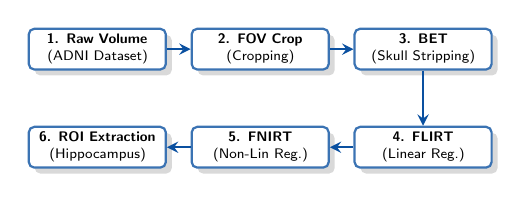
\begin{tikzpicture}[
        node distance=0.5cm and 0.3cm,
        font=\sffamily\tiny,
        stepbox/.style={rectangle, draw=techBlue!80, fill=white, thick, rounded corners=2pt, text width=1.6cm, align=center, inner sep=2pt, drop shadow={opacity=0.3}},
        arrow/.style={->, >=stealth, thick, techBlue, rounded corners=2pt}
    ]
        % Row 1
        \node[stepbox] (step1) {\textbf{1. Raw Volume}\\(ADNI Dataset)};
        \node[stepbox, right=of step1] (step2) {\textbf{2. FOV Crop}\\(Cropping)};
        \node[stepbox, right=of step2] (step3) {\textbf{3. BET}\\(Skull Stripping)};
        
        % Row 2
        \node[stepbox, below=0.7cm of step3] (step4) {\textbf{4. FLIRT}\\(Linear Reg.)};
        \node[stepbox, left=of step4] (step5) {\textbf{5. FNIRT}\\(Non-Lin Reg.)};
        \node[stepbox, left=of step5] (step6) {\textbf{6. ROI Extraction}\\(Hippocampus)};

        \draw[arrow] (step1) -- (step2);
        \draw[arrow] (step2) -- (step3);
        \draw[arrow] (step3.south) -- ++(0,-0.3) -| (step4.north);
        \draw[arrow] (step4) -- (step5);
        \draw[arrow] (step5) -- (step6);
    \end{tikzpicture}%
    }
    \caption{Six-step standardized MRI preprocessing pipeline utilizing FSL tools to extract the hippocampal ROI.}
    \label{fig:mri_pipeline}
\end{figure}

\subsubsection{Progressive Transfer Learning}
To prevent catastrophic forgetting and stabilize training on small datasets, a three-phase fine-tuning schedule is implemented:
\begin{itemize}
    \item \textbf{Phase 1 (Feature Extraction):} Backbone frozen, custom classifier head trained ($\eta = 10^{-4}$, 10 epochs).
    \item \textbf{Phase 2 (Shallow Tuning):} Unfreeze last 8 layers, train with low learning rate ($\eta = 10^{-5}$, 10 epochs).
    \item \textbf{Phase 3 (Deep Tuning):} Unfreeze last 10 layers, train for full adaptation ($\eta = 10^{-5}$, 20 epochs).
\end{itemize}

\subsubsection{Dual-Model Disjunction Fusion}
To mitigate false negatives in clinical diagnostics, the authors propose a logical disjunction (OR) fusion. Let $L_1$ be the binary prediction of the Base VGG16 (frozen backbone) and $L_2$ be the prediction of the Tuned VGG16:
\begin{equation}
    L_{final} = L_1 \lor L_2
\end{equation}
If either model flags the MRI as positive for AD, the final diagnosis is positive, increasing diagnostic sensitivity.

\begin{figure}[h]
    \centering
    \resizebox{0.9\linewidth}{!}{%
    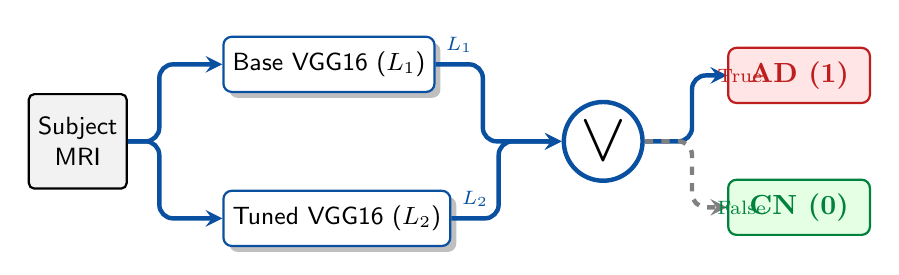
\begin{tikzpicture}[
        node distance=0.5cm and 0.8cm,
        font=\sffamily\small,
        input/.style={rectangle, draw=black, thick, fill=gray!10, minimum width=1.2cm, minimum height=1.2cm, rounded corners=2pt, align=center},
        model/.style={rectangle, draw=techBlue, thick, fill=white, minimum width=2.2cm, minimum height=0.7cm, rounded corners=3pt, drop shadow, align=center},
        gate/.style={circle, draw=techBlue, ultra thick, fill=white, minimum size=1.0cm, inner sep=0pt, align=center},
        outcome/.style={rectangle, draw=black, thick, minimum width=1.8cm, minimum height=0.7cm, rounded corners=3pt, font=\bfseries, align=center},
        arrow/.style={->, >=stealth, ultra thick, techBlue, rounded corners=5pt}
    ]
        \node[input] (mri) {Subject\\MRI};
        \node[model, above right=0.0cm and 1.2cm of mri] (m1) {Base VGG16 ($L_1$)};
        \node[model, below right=0.0cm and 1.2cm of mri] (m2) {Tuned VGG16 ($L_2$)};
        \coordinate (midpoint) at ($(m1.east)!0.5!(m2.east)$);
        \node[gate, right=1.5cm of midpoint] (or) {\Huge $\lor$};
        \node[outcome, above right=0.1cm and 1.2cm of or, draw=alertRed, fill=red!10, text=alertRed] (ad) {AD (1)};
        \node[outcome, below right=0.1cm and 1.2cm of or, draw=codeGreen, fill=green!10, text=codeGreen] (cn) {CN (0)};

        \draw[arrow] (mri.east) -- ++(0.4,0) |- (m1.west);
        \draw[arrow] (mri.east) -- ++(0.4,0) |- (m2.west);
        \draw[arrow] (m1.east) -- node[midway, above, font=\scriptsize] {$L_1$} ++(0.6,0) |- (or.west);
        \draw[arrow] (m2.east) -- node[midway, above, font=\scriptsize] {$L_2$} ++(0.6,0) |- (or.west);
        \draw[arrow] (or.east) -- ++(0.6,0) |- node[pos=0.7, right, font=\scriptsize, text=alertRed] {True} (ad.west);
        \draw[arrow, dashed, gray] (or.east) -- ++(0.6,0) |- node[pos=0.7, right, font=\scriptsize, text=codeGreen] {False} (cn.west);
    \end{tikzpicture}%
    }
    \caption{Dual-model logical disjunction (OR) fusion pipeline. By checking both models, it minimizes false negatives.}
    \label{fig:fusion_logic}
\end{figure}

\subsection{Experimental Performance \& Analysis}
Table \ref{tab:alzheimer_results} shows the performance metrics. The disjunction fusion achieves the highest accuracy of \highlight{89.87\%} and boosts diagnostic Sensitivity to \highlight{87.50\%} (+12.5\% over the base model), recovering 5 patients who were previously misdiagnosed. This comes with only a minor drop in Precision compared to the Tuned VGG16 model.

\begin{table}[h]
    \centering
    \caption{Performance results of VGG16 models and fusion strategy.}
    \label{tab:alzheimer_results}
    \resizebox{\linewidth}{!}{%
    \begin{tabular}{lcccc}
        \toprule
        \textbf{Model Strategy} & \textbf{Accuracy} & \textbf{Precision} & \textbf{Sensitivity} & \textbf{F1-Score} \\
        \midrule
        Base VGG16 ($L_1$) & 83.54\% & 90.91\% & 75.00\% & 82.19\% \\
        Tuned VGG16 ($L_2$) & 87.34\% & \textbf{94.12\%} & 80.00\% & 86.49\% \\
        \rowcolor{techBlue!10}
        \textbf{Fused VGG16 ($L_1 \lor L_2$)} & \textbf{89.87\%} & 92.11\% & \textbf{87.50\%} & \textbf{89.74\%} \\
        \bottomrule
    \end{tabular}
    }
\end{table}

\subsection{Advanced MLE/AIE Proposed Extensions}
While effective, the paper's methods use 2D networks for 3D MRI volumes and apply a naive binary OR logic that can increase false positives in noisier datasets. We propose three advanced extensions.

\subsubsection{1. 3D Swin UNETR Voxel-wise Modeling}
Instead of slice-wise 2D processing, we propose using a 3D Swin Transformer (Swin UNETR) \cite{swin_unetr_2022} to capture continuous volumetric spatial features. The input 3D MRI volume $X_{3D} \in \mathbb{R}^{H \times W \times D \times C}$ is projected into 3D voxel patches of size $P_h \times P_w \times P_d$. Self-attention is computed over local 3D windows:
\begin{equation}
    \text{Attention}(Q,K,V) = \text{Softmax}\left(\frac{QK^T}{\sqrt{d}} + B\right)V
\end{equation}
where $B \in \mathbb{R}^{N^2}$ is a 3D relative position bias. This models continuous spatial shrinkage of the hippocampus in 3D, avoiding spatial information loss.

\subsubsection{2. Multi-Modal Cross-Attention Fusion}
To improve diagnostic accuracy, we propose fusing the MRI imaging features with clinical tabular data (e.g., Mini-Mental State Examination (MMSE) scores, age, APOE-$\epsilon4$ genetic markers, and CSF amyloid-$\beta$ levels). 
Let $H_{img} \in \mathbb{R}^{N \times d}$ be the spatial image features and $H_{tab} \in \mathbb{R}^{M \times d}$ be the tabular features. We use a cross-attention layer to map the modalities:
\begin{align}
    Q &= H_{tab} W_q, \quad K = H_{img} W_k, \quad V = H_{img} W_v \\
    H_{fused} &= \text{Softmax}\left(\frac{Q K^T}{\sqrt{d}}\right) V \in \mathbb{R}^{M \times d}
\end{align}
The fused representation combines visual atrophy features with cognitive and genetic indicators before classification.

\subsubsection{3. Attention-based Multiple Instance Learning (AMIL)}
Instead of simple average-pooling to aggregate slice predictions, we propose modeling subject-level inference via Attention-based Multiple Instance Learning (AMIL) \cite{amil_ilse_2018}. A patient's MRI is treated as a "bag" of slices $H = \{h_1, \dots, h_N\}$. The bag embedding $Z$ is computed as:
\begin{equation}
    Z = \sum_{i=1}^N a_i h_i \quad \text{where } a_i = \frac{\exp(\mathbf{w}^T \tanh(\mathbf{V} h_i^T))}{\sum_{j=1}^N \exp(\mathbf{w}^T \tanh(\mathbf{V} h_j^T))}
\end{equation}
where $\mathbf{w} \in \mathbb{R}^{L \times 1}$ and $\mathbf{V} \in \mathbb{R}^{L \times D}$ are learnable parameters. The model automatically learns to weight key slices showing hippocampal atrophy, while ignoring uninformative peripheral slices.


% --- Section 4: LLM Code Review ---
% -----------------------------------------------------------------------------
% File: sections/04_llm_code_review.tex
% Description: Section 4 - LLMs as Code Review Agents
% -----------------------------------------------------------------------------

\section{Paper 3: LLMs as Code Review Agents}
\label{sec:llm_review}

\paperCard{LLMs as Code Review Agents: A Rapid Review and Experimental Evaluation with Human Expert Judges}{M. Kawalerowicz, M. Pietranik, K. St\k{e}pniak}{ICCCI 2025}

\subsection{Background and Research Motivation}
Quality assurance through code review is a vital phase of the software development lifecycle (SDLC), ensuring that code meets functional requirements, adheres to design principles, and is free from security vulnerabilities. However, manual code review by human developers is resource-intensive, time-consuming, and often becomes a bottleneck that slows down development velocity.

Traditional automated tools such as static analyzers and linters are limited to syntactic rules and pattern matching, failing to assess higher-level semantic properties like code readability, adherence to SOLID design principles (SRP, OCP, LSP, ISP, DIP), or the identification of complex security risks and architectural anti-patterns.

Recently, Large Language Models (LLMs) have been proposed as automated code review agents under the \highlight{LLM-as-a-Judge} paradigm. While LLMs are significantly cheaper and faster than human reviewers, assessing their alignment with human expert consensus and understanding their biases is crucial before deploying them in production code review pipelines. Key questions include: How well do LLMs correlate with senior developer evaluations? Which metrics do they excel at? And what is the cost-benefit trade-off between accuracy and API expenses?

\subsection{Paper Objectives}
The paper conducts a comparative evaluation of LLM-generated code quality assessments against human expert judgments. The specific objectives include:
\begin{itemize}
    \item Designing a parallel evaluation framework where both LLM agents and human experts independently score the same code corpus.
    \item Evaluating 6 LLMs (Claude 3.5 Sonnet, Claude 3.5 Haiku, GPT-4o-mini, Mistral Large, Ministral-8b, Falcon3-7B) against 3 human software developers with 5--15 years of industry experience.
    \item Measuring alignment using statistically rigorous non-parametric methods (Shapiro-Wilk test, Spearman rank correlation).
    \item Providing a cost-benefit analysis to determine which LLM offers the best accuracy-to-cost ratio for production deployment.
\end{itemize}

\subsection{Proposed Method}

\subsubsection{Parallel Evaluation Framework}
The study establishes a controlled experimental framework where both human experts and LLM agents independently evaluate the same set of code files. A custom evaluation platform is developed for human reviewers, while LLMs receive structured prompts with identical evaluation criteria.

\begin{figure}[h]
    \centering
    \resizebox{0.95\textwidth}{!}{%
    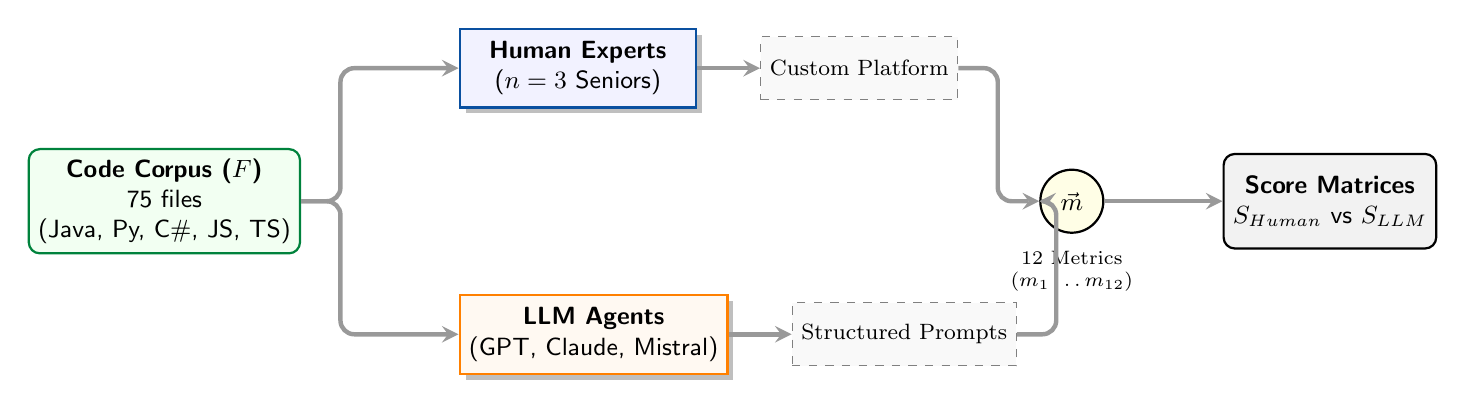
\begin{tikzpicture}[
        node distance=0.5cm and 1.0cm,
        font=\sffamily\small,
        corpus/.style={rectangle, draw=codeGreen, fill=green!5, thick, minimum width=2.5cm, minimum height=1.2cm, align=center, rounded corners},
        actor/.style={rectangle, draw=black, thick, fill=white, minimum width=3cm, minimum height=1.0cm, align=center, drop shadow},
        process/.style={rectangle, draw=gray, dashed, fill=gray!5, minimum width=2.5cm, minimum height=0.8cm, align=center, font=\footnotesize},
        metric/.style={circle, draw=black, fill=yellow!10, thick, inner sep=2pt, minimum size=0.8cm},
        arrow/.style={->, >=stealth, ultra thick, gray!80, rounded corners=5pt}
    ]
        \node[corpus] (input) {\textbf{Code Corpus ($F$)}\\75 files\\(Java, Py, C\#, JS, TS)};
        \node[actor, above right=0.5cm and 2.0cm of input, draw=techBlue, fill=blue!5] (human) {\textbf{Human Experts}\\($n=3$ Seniors)};
        \node[actor, below right=0.5cm and 2.0cm of input, draw=orange, fill=orange!5] (llm) {\textbf{LLM Agents}\\(GPT, Claude, Mistral)};
        \node[process, right=0.8cm of human] (platform) {Custom Platform};
        \node[process, right=0.8cm of llm] (prompt) {Structured Prompts};
        \coordinate (midpoint) at ($(platform)!0.5!(prompt)$);
        \node[metric, right=2.0cm of midpoint, align=center] (metrics) {$\vec{m}$};
        \node[below=0.1cm of metrics, font=\scriptsize, align=center] {12 Metrics\\($m_1 \dots m_{12}$)};
        \node[corpus, right=1.5cm of metrics, fill=gray!10, draw=black] (output) {\textbf{Score Matrices}\\$S_{Human} \text{ vs } S_{LLM}$};
        \draw[arrow] (input.east) -- ++(0.5,0) |- (human.west);
        \draw[arrow] (input.east) -- ++(0.5,0) |- (llm.west);
        \draw[arrow] (human) -- (platform);
        \draw[arrow] (llm) -- (prompt);
        \draw[arrow] (platform.east) -- ++(0.5,0) |- (metrics.west);
        \draw[arrow] (prompt.east) -- ++(0.5,0) |- (metrics.west);
        \draw[arrow] (metrics) -- (output);
    \end{tikzpicture}%
    }
    \caption{Methodology flow of the parallel code quality evaluation framework.}
    \label{fig:llm_flow}
\end{figure}

\subsubsection{Code Corpus and Evaluators}
\begin{itemize}
    \item \textbf{Dataset:} 75 source code files in Java, C\#, Python, JavaScript, and TypeScript, selected to represent varying levels of code quality from poor to excellent.
    \item \textbf{Human evaluators:} 3 senior software developers with 5--15 years of industry experience, each independently scoring all 75 files.
    \item \textbf{LLM evaluators:} 6 LLMs of varying sizes and capabilities: Claude 3.5 Sonnet, Claude 3.5 Haiku, GPT-4o-mini, Mistral Large, Ministral-8b, and Falcon3-7B.
\end{itemize}

\subsubsection{Code Quality Metrics}
Each code file is scored on a scale of 1--10 across 12 quality metrics:
\begin{itemize}
    \item \textbf{Comments} ($m_1$), \textbf{DIP} ($m_2$), \textbf{Formatting} ($m_3$), \textbf{ISP} ($m_4$), \textbf{KISS} ($m_5$), \textbf{LSP} ($m_6$)
    \item \textbf{Naming} ($m_7$), \textbf{OCP} ($m_8$), \textbf{Performance} ($m_9$), \textbf{DRY/Repetition} ($m_{10}$), \textbf{Safety} ($m_{11}$), \textbf{SRP} ($m_{12}$)
\end{itemize}

\subsubsection{Statistical Analysis Pipeline}
The study establishes a rigorous statistical pipeline to validate its findings:
\begin{enumerate}
    \item \textbf{Normality Check:} The Shapiro-Wilk test is performed on all score distributions. The resulting $p$-values are less than $0.05$ ($p < \alpha$), indicating that scores do not follow a normal distribution.
    \item \textbf{Correlation Metric:} Because the data is non-normal, the non-parametric \highlight{Spearman Rank Correlation} ($\rho$) is used:
    \begin{equation}
        \rho = 1 - \frac{6 \sum d_i^2}{n(n^2 - 1)}
    \end{equation}
    where $d_i$ is the difference between ranks.
    \item \textbf{Ground Truth Modeling:} Human developer consensus is established as the ground truth baseline:
    \begin{equation}
        GT(f_i) = \text{Median}(S_{Human1}(f_i), S_{Human2}(f_i), S_{Human3}(f_i))
    \end{equation}
\end{enumerate}

\subsection{Experiments and Results}

\subsubsection{Spearman Correlation with Human Consensus}
Table~\ref{tab:llm_metrics} presents the Spearman correlation of each LLM with the human consensus baseline across all 12 quality metrics.

\begin{table}[h]
    \centering
    \caption{Spearman correlation ($\rho$) of LLM agents with human consensus.}
    \label{tab:llm_metrics}
    \resizebox{\linewidth}{!}{%
    \begin{tabular}{lcccccc}
        \toprule
        \textbf{Metric} & \textbf{Sonnet} & \textbf{GPT-4o-m} & \textbf{Mistral L} & \textbf{Haiku} & \textbf{Min-8b} \\
        \midrule
        $m_1$ (Comm.) & \textbf{0.71} & 0.64 & 0.57 & 0.62 & 0.43 \\
        $m_2$ (DIP)   & \textbf{0.83} & 0.58 & 0.54 & 0.50 & 0.30 \\
        $m_3$ (Format)& \textbf{0.71} & 0.66 & 0.60 & 0.65 & 0.48 \\
        $m_4$ (ISP)   & \textbf{0.90} & 0.81 & 0.76 & 0.44 & 0.28 \\
        $m_5$ (KISS)  & \textbf{0.85} & 0.76 & 0.79 & 0.66 & 0.59 \\
        $m_6$ (LSP)   & \textbf{0.88} & 0.74 & 0.69 & 0.28 & 0.17 \\
        $m_7$ (Name)  & 0.80 & 0.72 & \textbf{0.81} & 0.70 & 0.59 \\
        $m_8$ (OCP)   & \textbf{0.79} & 0.65 & 0.73 & 0.77 & 0.57 \\
        $m_9$ (Perf)  & 0.73 & 0.66 & \textbf{0.73} & 0.53 & 0.58 \\
        $m_{10}$ (DRY)& \textbf{0.87} & 0.79 & 0.87 & 0.78 & 0.59 \\
        $m_{11}$ (Safe)& 0.76 & 0.75 & \textbf{0.77} & 0.70 & 0.69 \\
        $m_{12}$ (SRP) & \textbf{0.86} & 0.78 & 0.85 & 0.71 & 0.63 \\
        \bottomrule
    \end{tabular}
    }
\end{table}

Detailed analysis of the results:
\begin{itemize}
    \item \textbf{Claude 3.5 Sonnet} achieves the highest alignment with human consensus in \highlight{9 out of 12 metrics}, demonstrating particularly strong performance on complex SOLID design principles: ISP ($\rho = 0.90$), LSP ($\rho = 0.88$), DRY ($\rho = 0.87$), and SRP ($\rho = 0.86$).
    \item \textbf{Mistral Large} achieves the best scores in 3 metrics: Naming ($\rho = 0.81$), Performance ($\rho = 0.73$), and Safety ($\rho = 0.77$), suggesting strength in surface-level code evaluation.
    \item \textbf{Smaller models} (Ministral-8b, Falcon3-7B) show significantly lower correlations across all metrics, particularly in complex design principles like LSP ($\rho = 0.17$) and ISP ($\rho = 0.28$), indicating that model size plays a crucial role in understanding abstract software engineering concepts.
    \item \textbf{GPT-4o-mini} provides consistently moderate correlations ($\rho \approx 0.65$--$0.81$) across all metrics, positioning it as a balanced mid-tier option.
\end{itemize}

\subsubsection{Cost-Benefit Analysis}
Table~\ref{tab:cost_analysis} presents the cost comparison for evaluating the full corpus of 75 code files.

\begin{table}[h]
    \centering
    \caption{Cost comparison for evaluating 75 code files.}
    \label{tab:cost_analysis}
    \small
    \begin{tabular}{lrc}
        \toprule
        \textbf{Evaluator} & \textbf{Cost} & \textbf{Ratio} \\
        \midrule
        Claude 3.5 Sonnet & \$8.52 & 31.6$\times$ \\
        Claude 3.5 Haiku & \$1.66 & 6.1$\times$ \\
        \rowcolor{techBlue!10}
        \textbf{GPT-4o-mini} & \textbf{\$0.27} & \textbf{1.0$\times$} \\
        Human Experts (1--2 days) & \$200--400+ & 740--1480$\times$ \\
        \bottomrule
    \end{tabular}
\end{table}

Key findings from the cost analysis:
\begin{itemize}
    \item While Claude 3.5 Sonnet is the most accurate LLM, it costs \$8.52 per evaluation cycle, making it 31.6 times more expensive than GPT-4o-mini.
    \item \textbf{GPT-4o-mini} provides the best cost-to-accuracy ratio at only \$0.27 per cycle with correlations averaging $\rho \approx 0.75$, making it highly suitable for high-volume production pipelines.
    \item Human experts remain orders of magnitude more expensive (740--1480$\times$) while requiring 1--2 days per evaluation cycle, underscoring the economic case for LLM-assisted code review.
\end{itemize}

\subsection{Conclusion and Contributions}
The paper provides a systematic experimental comparison of LLM code review capabilities against human expert baselines.

Key contributions of the paper:
\begin{itemize}
    \item Establishes a rigorous parallel evaluation framework with statistically validated methodology (Shapiro-Wilk normality test, Spearman rank correlation).
    \item Demonstrates that Claude 3.5 Sonnet achieves the highest alignment with human expert consensus in 9 out of 12 code quality metrics, particularly in complex design principles.
    \item Reveals that model size strongly correlates with the ability to evaluate abstract software engineering concepts (SOLID principles).
    \item Provides a practical cost-benefit analysis showing that GPT-4o-mini offers the optimal balance between accuracy and cost for production-scale code review.
    \item Highlights that while LLMs cannot fully replace human reviewers, they can serve as effective first-pass screening tools, significantly reducing the workload on senior developers.
\end{itemize}


% --- Section 5: Conclusion ---
% -----------------------------------------------------------------------------
% File: sections/05_conclusion.tex
% Description: Section 5 - Overall Conclusion
% -----------------------------------------------------------------------------

\section{Overall Conclusion}
\label{sec:conclusion}

This report has presented a comprehensive analysis and synthesis of three state-of-the-art research papers presented at ICCCI 2025, addressing key challenges in computer-aided diagnostics and automated software engineering.

\subsection{Summary of Key Findings}

\begin{enumerate}
    \item \textbf{Leukemia Detection (YOLOv11 + GCLI):} The GCLI module effectively replaces the C2PSA self-attention block, achieving the highest mAP50-95 of 25.1\% while reducing over 11\% of parameters. The module's strength lies in its ability to capture global--local feature interactions without dimensionality reduction, making it a lightweight yet powerful attention mechanism for cell-level object detection.

    \item \textbf{Alzheimer Diagnosis (VGG16 Fusion):} The dual-model disjunction fusion strategy achieves 89.87\% accuracy and 87.50\% sensitivity, recovering 5 previously missed AD patients. The paper makes an important methodological contribution by enforcing subject-wise data splitting to eliminate the data leakage problem prevalent in prior studies.

    \item \textbf{LLM Code Review:} Claude 3.5 Sonnet demonstrates the highest alignment with human expert consensus (9/12 metrics), while GPT-4o-mini provides the best cost-to-accuracy ratio at 31.6$\times$ lower cost. The study establishes that LLMs can serve as effective first-pass code review tools, though they cannot yet fully replace senior human reviewers.
\end{enumerate}

\subsection{Cross-Domain Observations}

Comparing the three research domains reveals important parallels and contrasts:
\begin{itemize}
    \item \textbf{Data Integrity:} Both medical imaging and code review face data integrity challenges, though manifested differently. In medical imaging, data leakage (sharing patient slices between train/test splits) artificially inflates performance metrics. In code review, the challenge is context limitation: single-file LLM analysis misses project-level dependencies, yielding incomplete assessments.

    \item \textbf{Sensitivity vs. Precision Trade-off:} In clinical CAD systems, sensitivity is the primary safety metric because false negatives delay critical treatment. The VGG16 fusion paper addresses this through logical disjunction ($L_1 \lor L_2$). Conversely, in software engineering, developers are sensitive to ``linter fatigue'' from excessive false positives. Review systems must balance precision with API costs, making GPT-4o-mini a viable production option.

    \item \textbf{Lightweight vs. Heavyweight Approaches:} All three papers demonstrate that domain-specific, targeted solutions can outperform heavyweight general-purpose methods. GCLI replaces expensive self-attention with lightweight 1D convolutions. Progressive transfer learning adapts pre-trained models without full retraining. And carefully prompted LLMs can approximate human-level code assessment at a fraction of the cost.
\end{itemize}

\subsection{Limitations and Future Directions}
Despite the promising results, each paper presents opportunities for further development:
\begin{itemize}
    \item The GCLI module was evaluated only on YOLOv11; testing on other YOLO variants and two-stage detectors would strengthen generalizability claims.
    \item The VGG16 fusion approach uses 2D slice processing on inherently 3D MRI volumes; 3D architectures could capture volumetric spatial information more effectively.
    \item The LLM code review study evaluates single-file contexts; extending to project-level analysis with dependency-aware prompting could significantly improve SOLID principle assessments.
\end{itemize}

These findings collectively underscore that while deep learning models and LLMs provide strong performance baselines, achieving robust real-world deployment requires careful attention to data integrity, domain-specific architectural design, and rigorous statistical validation.


% --- Bibliography ---
\small
\printbibliography

\end{document}
